%
% 3dimagetemplate.tex
%
% (c) 2018 Prof Dr Andreas Müller, Hochschule Rapperswil
%
\documentclass[tikz]{standalone}
\usepackage{times}
\usepackage{amsmath}
\usepackage{txfonts}
\usepackage[utf8]{inputenc}
\usepackage{graphics}
\usetikzlibrary{arrows,intersections,math}
\usepackage{ifthen}
\begin{document}

\newboolean{showgrid}
\setboolean{showgrid}{false}
\def\breite{7}
\def\hoehe{8}

\begin{tikzpicture}[>=latex,thick]

% Povray Bild
\node at (0,0) {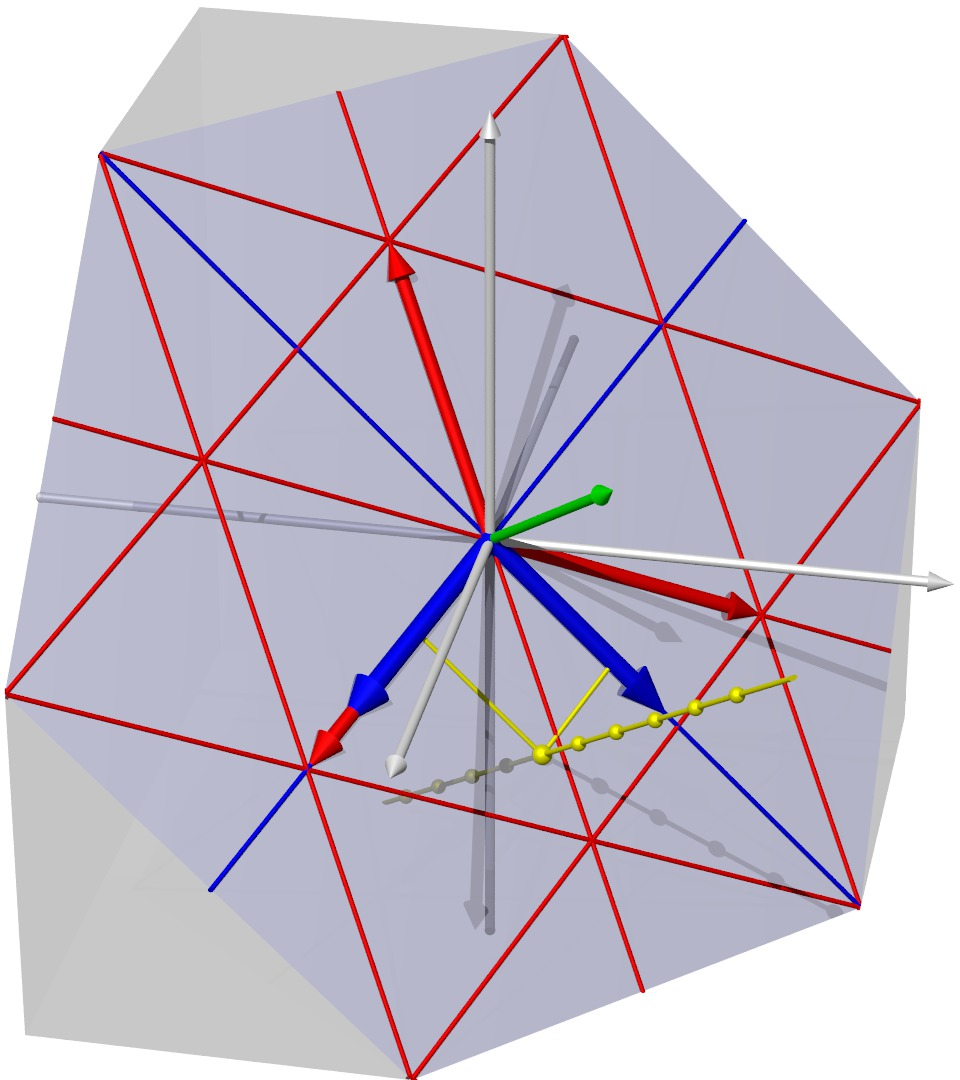
\includegraphics[width=14cm]{tri.jpg}};

% Gitter
\ifthenelse{\boolean{showgrid}}{
\draw[step=0.1,line width=0.1pt] (-\breite,-\hoehe) grid (\breite, \hoehe);
\draw[step=0.5,line width=0.4pt] (-\breite,-\hoehe) grid (\breite, \hoehe);
\draw                            (-\breite,-\hoehe) grid (\breite, \hoehe);
\fill (0,0) circle[radius=0.05];
}{}

\node at (-1.5,-3.4) {$\hat{v}_1$};
\node at (6.7,-0.3) {$\hat{v}_2$};
\node at (-0.1,6.2) {$\hat{v}_3$};

\node at (2.1,0.8) {$n$};

\node at (-2.8,-3.4) {$b'_1$};
\node at (4.15,-0.7) {$b'_2$};
\node at (-1.5,4.2) {$b'_3$};

\node at (0.9, -3.5) {$v'$};
\node at (2,-3.1) {$w$};

\end{tikzpicture}

\end{document}

